% Chapter 1

\chapter{Introducción General} % Main chapter title

\label{chapter1} % For referencing the chapter elsewhere, use \ref{Chapter1} 
\label{IntroGeneral}

%----------------------------------------------------------------------------------------

% Define some commands to keep the formatting separated from the content 
\newcommand{\keyword}[1]{\textbf{#1}}
\newcommand{\tabhead}[1]{\textbf{#1}}
\newcommand{\code}[1]{\texttt{#1}}
\newcommand{\file}[1]{\texttt{\bfseries#1}}
\newcommand{\option}[1]{\texttt{\itshape#1}}
\newcommand{\grados}{$^{\circ}$}

%----------------------------------------------------------------------------------------

%\section{Introducción}

%----------------------------------------------------------------------------------------

En este capítulo se realiza una introducción al concepto de Internet de las Cosas, se describe la motivación del trabajo realizado y se presentan sus objetivos y alcance.

\section{Internet de las Cosas{}}

Desde la aparición de Internet a finales del siglo pasado, ha quedado demostrado lo útil que es contar con un dispositivo capaz de conectarse a la red. Los beneficios de que una computadora o un teléfono inteligente puedan conectarse a Internet son evidentes, y esos beneficios también se encuentran presentes al conectar cualquier otro objeto a Internet, y es allí donde surge el concepto de Internet de las Cosas (IoT, por sus siglas en inglés correspondientes a \emph{Internet of Things}).

La Internet de las Cosas consiste en extender el potencial de Internet y la conectividad más allá de las computadoras y celulares, e incorporar a todos los objetos (cosas) de la vida cotidiana y que se encuentran presentes en el entorno de una persona. Así se permite tanto la comunicación e interacción entre sí de estos objetos, como así también el monitoreo y control en forma remota.

El concepto de \enquote{cosa} es sumamente amplio, ya que contempla desde lámparas, cerraduras y termostatos en el hogar, hasta maquinaria industrial y sistemas de riego para agricultura, pasando por vehículos autónomos, sistemas de iluminación y sensores para estacionamiento público en una ciudad. El objeto conectado incluso puede ser un monitor cardíaco en el interior de una persona o un chip insertado en un animal de granja. Gracias a la existencia de sensores y microcontroladores cada vez más potentes, más pequeños y de menor costo, es posible lograr que prácticamente cualquier dispositivo forme parte del ecosistema IoT.

Los beneficios que la Internet de las Cosas ofrece tanto a empresas como a personas individuales son innumerables. Desde un punto de vista económico, les da la posibilidad a las empresas de conocer y monitorear mejor sus procesos, para así hacerlos más eficientes y posibilitar mejores tomas de decisiones y acciones como mantenimiento predictivo de maquinaria. Todo eso se traduce en definitiva en un ahorro de dinero y tiempo para la organización. Con respecto a un individuo particular, la Internet de las Cosas le permite mejorar su calidad de vida y su comodidad en el día a día con automatizaciones en el hogar (domótica), como así también beneficios a la salud con, por ejemplo, implantes inteligentes que permiten un cuidadoso monitoreo.

Las empresas, las personas y el mercado en general hace ya varios años que se han dado cuenta de la importancia de la Internet de las Cosas. Es prueba de ello la gran cantidad de dispositivos conectados que existen, y las proyecciones que indican que estos números seguirán aumentando notablemente. En 2017 ya había 27 mil millones de dispositivos IoT conectados, cifra que aumentará a un ritmo de un 12\% anual hasta llegar a 125 mil millones para 2030 \citep{1}. Por otra parte, en la figura \ref{fig:iot_market} se puede observar cómo el mercado mundial de la Internet de las Cosas ya maneja cantidades de dinero superiores a los USD 200.000.000.000, y cómo esa cifra aumentará sustancialmente a lo largo de los próximos años \citep{2}, lo cual supone una enorme oportunidad de negocio para muchas empresas.

\begin{figure}[h]
\centering
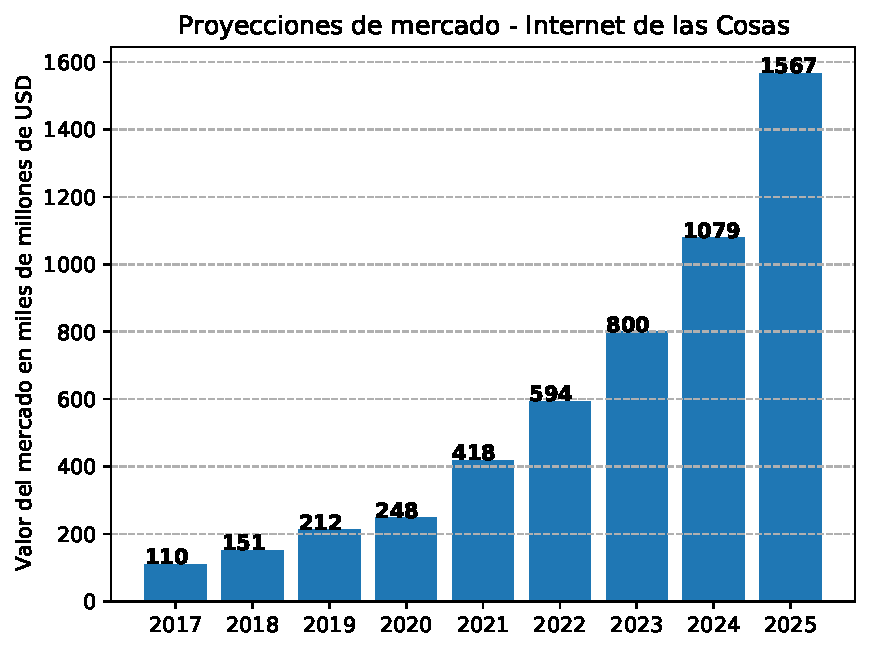
\includegraphics[width=\textwidth]{./Figures/iot_market_projection.pdf}
\caption[Proyecciones del valor de mercado a nivel mundial de la Internet de las Cosas.]{Proyecciones del valor de mercado a nivel mundial de la Internet de las Cosas.\footnotemark}
\label{fig:iot_market}
\end{figure}

\footnotetext{Gráfico replicado en base al que se muestra en \url{https://www.statista.com/statistics/976313/global-iot-market-size/}.}


Por último, un punto que a menudo es pasado por alto al momento de hablar de la Internet de las Cosas, son todos los problemas asociados a la seguridad y la privacidad. Tener un mayor número de dispositivos conectados, muchos de los cuales recolectan información sumamente sensible, expande la superficie de ataque considerablemente, y deja tanto a empresas como a personas más vulnerables frente a posibles ciberdelincuentes. Existen incontables ejemplos de vulnerabilidades en dispositivos IoT que salieron a la luz, como una gigantesca \emph{botnet} formada por dispositivos IoT \citep{3}, televisores inteligentes que espían conversaciones privadas \citep{4}, e incluso ataques dirigidos a dispositivos conectados en entornos industriales \citep{5}. Estos hechos ocurren principalmente porque la seguridad y la privacidad a menudo son vistas como costos extra en los que no vale la pena incurrir. Incluso en ocasiones la propia empresa utiliza de manera poco ética esos agujeros de seguridad para obtener datos de los usuarios y sacar algún tipo de provecho económico a partir de ellos.

Las consecuencias de una falla de seguridad en un dispositivo IoT pueden ser muy graves, por lo que al momento de desarrollar una solución en el segmento del Internet de las Cosas, los aspectos de seguridad deben ser tenidos en consideración desde un principio, aún cuando ello implique desarrollar un producto más costoso o complejo.

\section{Estado del arte{}}
\label{sec:estado_del_arte}

En la actualidad, existe una enorme cantidad de dispositivos conectados que pertenecen a muy diversos ámbitos, por lo que resultaría poco práctico brindar un panorama general del estado del arte en todos ellos. Por lo tanto, el foco estará en aquellos productos que ofrezcan soluciones orientadas a dispositivos que ya cuentan con cierto nivel de ''inteligencia'' (como maquinaria industrial/agrícola o artefactos del hogar), a los fines de dotarlos de conectividad y de todo un entorno que permita procesar y analizar los datos generados por ellos.

Por un lado, existen numerosas plataformas que solamente ofrecen la etapa de procesamiento, análisis y visualización de datos. Estas plataformas asumen que el cliente cuenta con el hardware necesario para enviarles la información relevante, y ellas se encargan de analizarla y presentarla de manera conveniente mediante tableros o \emph{dashboards}, que le permiten al usuario ver el estado de los dispositivos y actuar sobre ellos. La mayoría de estas plataformas poseen características similares tales como administración de dispositivos, visualización de datos y soporte a múltiples protocolos de comunicación. Algunos ejemplos de esta clase de plataformas son ThingBoard \citep{7}, Thinger \citep{8} y Ubidots \citep{9}, además de los servicios específicamente orientados a IoT de Amazon Web Services, de Google Cloud Platform y de Microsoft Azure.  

Por otra parte, existen también plataformas de hardware que ofrecen soluciones genéricas de conectividad, junto con plataformas para analizar y visualizar los datos obtenidos, con características similares a las mencionadas anteriormente.

En este último segmento hay diferentes grados de especialización. Por ejemplo, existen empresas que ofrecen soluciones orientadas exclusivamente al ámbito industrial, como ThingWorx de la empresa PTC \citep{10}, mientras que otras brindan soluciones más genéricas con una plataforma de hardware y un entorno de análisis y visualización, como el caso de Particle (figura \ref{fig:particle_iot}) \citep{11}.

\begin{figure}[h]
\centering
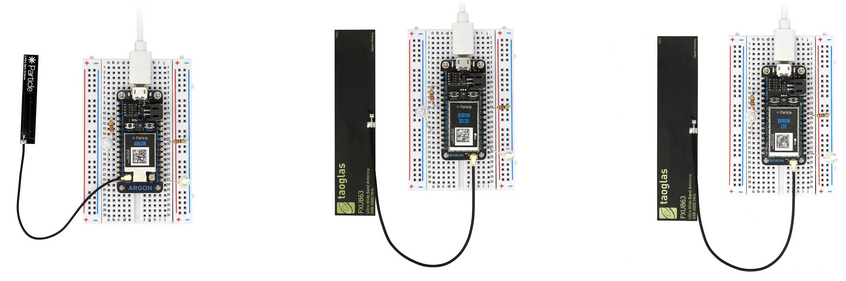
\includegraphics[scale=0.4]{./Figures/particle_iot.png}
\caption[Plataformas de hardware ofrecidas por Particle.]{Plataformas de hardware ofrecidas por Particle.\footnotemark}
\label{fig:particle_iot}
\end{figure}

\footnotetext{Imagen extraída de \url{https://store.particle.io/pages/prototyping-hardware}.}


\section{Motivación{}}

Un sector fundamental en el ámbito del Internet de las Cosas es el de la domótica, es decir el conjunto de tecnologías que permite el control y la automatización inteligente de una vivienda, a los fines de lograr una gestión eficiente y brindar mayor comodidad y seguridad a quienes la habitan \citep{6}.

A su vez, dentro de la domótica, un campo de especial interés es el de los electrodomésticos inteligentes (o \emph{smart appliances}), tales como televisores, heladeras, hornos, lavarropas o microondas. 

Una característica primordial de un electrodoméstico inteligente es su capacidad de
estar conectado y ser manejado o accedido de forma remota, ya sea mediante una plataforma web, una aplicación en el celular, comandos de voz o cualquier otro medio. Esta capacidad brinda grandes ventajas con respecto a un artefacto convencional, ya que no solamente ofrece una mayor comodidad al momento de usarlo, sino que también permite programar acciones (como preparar un café a una determinada hora) y ahorrar energía al hacer más eficiente su uso.

Actualmente existen ya en el mercado numerosos ejemplos de electrodomésticos inteligentes que permiten llevar a cabo diferentes acciones:
\begin{itemize}
	\item Encender el horno mediante un comando de voz, incluso con integración con los asistentes de voz más comunes.
	\item Consultar el contenido de la heladera mediante una aplicación en el celular.
	\item Recibir una notificación cuando el ciclo de lavado del lavarropas finaliza.
	\item Diagnosticar automáticamente la causa de una falla.
\end{itemize}

Gracias a las ventajas que ofrecen, la demanda de electrodomésticos inteligentes es cada vez más mayor, por lo que aquellas empresas o fabricantes que no se modernicen y comiencen a incorporar características \emph{smart} a sus dispositivos, se encontrarán en clara desventaja
al competir en el mercado con aquellas que sí lo hagan.

Como se puede apreciar en la sección \ref{sec:estado_del_arte}, existen ya en el mercado numerosas soluciones orientadas a la Internet de las Cosas. Cada una de ellas ofrece diferentes características y cubre diferentes mercados. Dentro de las soluciones que ofrecen una plataforma tanto de hardware como de software, no existe un sector consolidado que esté orientado a dotar de conectividad a electrodomésticos en el hogar, y es allí donde surge la importancia del presente trabajo. Lo que se busca es cubrir justamente ese sector y ofrecer una solución personalizada a los fabricantes para que puedan lograr que los electrodomésticos que ya fabrican se conviertan en electrodomésticos inteligentes.


\section{Objetivos y alcance{}}

\subsection{Objetivos generales}

El objetivo general del presente trabajo es el diseño e implementación de un módulo capaz de dotar de conectividad WiFi y Bluetooth a un electrodoméstico convencional. Para ello, el módulo debe tener la capacidad de comunicarse con la placa del propio equipo y de recibir/enviar información a un servidor en la nube, a los fines de permitirle al usuario final un manejo remoto del aparato y conocer su estado, como así también enviar información de uso al fabricante. 

El módulo no está destinado directamente al usuario final del electrodoméstico, sino a empresas o fabricantes que busquen incorporar características inteligentes a sus electrodomésticos.

A grandes rasgos, desde el punto de vista del usuario final, se debe permitir:
\begin{itemize}
	\item Enviar por WiFi o Bluetooth un comando al electrodoméstico que dispare una acción en él, como iniciar la cocción en un horno o el lavado en un lavarropas.
	\item Conocer el estado del electrodoméstico mediante la recepción de información por WiFi o Bluetooth.
\end{itemize}

Por otra parte, desde el punto de vista del fabricante del electrodoméstico se debe permitir:
\begin{itemize}
	\item Recibir y almacenar información acerca del estado de todos los dispositivos (si están o o no conectados, y en qué estado de ejecución se encuentran).
	\item Analizar y visualizar de manera conveniente la información de estado de los dispositivos a lo largo del tiempo.
\end{itemize}

\subsection{Alcance}

El presente trabajo incluye los siguientes aspectos:

\begin{enumerate}
	\item Análisis, investigación y elección del hardware a utilizar en el módulo.
	\item Implementación del firmware del sistema.
	\item Comunicación con un microcontrolador que emule el comportamiento del electrodoméstico.
	\item Desarrollo de una interfaz web mediante una plataforma ya existente, que permita enviarle comandos al electrodoméstico emulado.
	\item Implementación de un entorno en la nube que permita analizar y visualizar los datos de los diferentes electrodomésticos conectados.
\end{enumerate}

Es de especial importancia el punto 3 de la lista, en el que se define explícitamente que, a los fines de agilizar considerablemente el tiempo de desarrollo del trabajo, el prototipo no se utilizará en un electrodoméstico real. La interacción con él se emula mediante la comunicación con otro microcontrolador, que actúa como la placa de control del electrodoméstico: imita su comportamiento y sus respuestas ante diferentes estímulos.

En línea con el párrafo anterior, el presente trabajo no incluye lo siguiente:

\begin{enumerate}
	\item Integración del prototipo a diferentes electrodomésticos/marcas con distintos tipos de
comunicación serie y funcionalidades.
	\item Desarrollo de una aplicación móvil desde la cual interactuar por Bluetooth con el módulo.
	\item Diseño y fabricación de un circuito impreso. Para el trabajo se utiliza una placa de prototipo ya existente que incluye el hardware seleccionado.
\end{enumerate}






















 